\documentclass[3pt,twocolumn]{elsarticle}
\usepackage[spanish]{babel}
\usepackage[utf8]{inputenc}
\usepackage[hidelinks]{hyperref}
\usepackage{graphics}
\usepackage{graphicx}
\usepackage{blindtext, rotating}
\usepackage{adjustbox}
\usepackage{epsfig}
\usepackage{amssymb}
\usepackage{amsmath}
\usepackage{amsthm}
\usepackage{lineno}
\usepackage{tikz}
\usepackage{float}
\usepackage{subcaption}
\usepackage{amssymb, amsmath}
\usetikzlibrary{shapes,arrows}
\usepackage{pstricks,pst-node,pst-tree}
%\bibliographystyle{elsarticle-num}

\makeatletter
\renewenvironment{abstract}{\global\setbox\absbox=\vbox\bgroup
\hsize=\textwidth\def\baselinestretch{1}%
\noindent\unskip\textbf{Resumen} 
\par\medskip\noindent\unskip\ignorespaces}
{\egroup}

\def\keyword{%
\def\sep{\unskip, }%
\def\MSC{\@ifnextchar[{\@MSC}{\@MSC[2000]}}
\def\@MSC[##1]{\par\leavevmode\hbox {\it ##1~MSC:\space}}%
\def\PACS{\par\leavevmode\hbox {\it PACS:\space}}%
\def\JEL{\par\leavevmode\hbox {\it JEL:\space}}%
\global\setbox\keybox=\vbox\bgroup\hsize=\textwidth
\normalsize\normalfont\def\baselinestretch{1}
\parskip\z@
\noindent\textit{Palabras clave: } 
\raggedright 
\ignorespaces}

\biboptions{longnamesfirst,comma}

\usepackage{etoolbox}
\makeatletter
\def\ps@pprintTitle{%
     \let\@oddhead\@empty
     \let\@evenhead\@empty
     \def\@oddfoot{\footnotesize\itshape
        \ifx\@journal\@empty Simulación computacional de nanomateriales  % <--- Edit as necessary
       \else\@journal\fi\hfill\today}%
     \let\@evenfoot\@oddfoot}

\makeatother
\begin{document}

\twocolumn[
\begin{@twocolumnfalse}

\begin{frontmatter}
\title{Modelo de análisis térmico en estructuras cristalinas}
\author{Samaniego, E.}
\address{Posgrado en Maestría en Ciencias de la Ingeniería con Orientación en Nanotecnología.}
\address{Facultad de Ingeniería Mecánica y Eléctrica, Universidad Autónoma de Nuevo León}

\begin{abstract}
Se realiza un estudio de el comportamiento de las aleaciones de un material puro con cerámicos, polímeros y conductores con el fin de ver que pasa con la conductividad térmica principalmente si llega al punto de fusión dependiendo con que partículas se dope y la manera en que se haga la aleación ya sea distribuida en el material o como una capa superficial para analizar la eficiencia térmica en diferentes grados de temperatura y ver que es preferible, y a su vez ver que ocurre con la conductividad eléctrica del propio material.
Es comprobado gráficamente que un mejor comportamiento tanto térmico como de flujo eléctrico es visto en los materiales aleados poliméricamente ya que se encuentran en un punto medio entre los cerámicos que son completamente aislantes y la plata que es un material conductor.
\end{abstract}

\begin{keyword}
Conductividad térmica \sep punto de fusión \sep aleación \sep flujo eléctrico. 
\end{keyword}

\end{frontmatter}
\end{@twocolumnfalse}
]

\section{Introducción}\label{intr}
El estudio de la conductividad térmica en los materiales es de suma importancia para aplicarse en diferentes situaciones para el desarrollo de nuevos materiales para conocer ciertas características de algunas partículas. Las propiedades mecánicas de los materiales pueden controlarse por la adiciones de defecto puntuales como átomos sustitucionales e intersticiales. Particularmente el caso de los metales, los defectos puntuales distorsionan el arreglo atómico en la red, interfiriendo con el movimiento o deslizamiento de las dislocaciones.

La conducción se produce por cesión de energía entre partículas contiguas (vibraciones reticulares) también se debe al movimiento de traslación de los electrones libres \cite{book2}.
La conducción es el único mecanismo de transmisión del calor posible en los medios sólidos. Cuando en estos cuerpos existe un gradiente de temperatura, el calor se transmite de la región de mayor a la de menor temperatura. El flujo real de calor depende de la conductividad térmica, que es una propiedad física del cuerpo. 
Para la integración del estudio térmico en estructuras cristalinas con simulación computacional, es basado en el concepto teórico en que las partículas de un elemento tienen cierta conductividad térmica que puede ser modificada con la adición de otros elementos con menos conductividad térmica para que el material base aumente su resistencia a la temperatura y como afecta su conductividad eléctrica, siendo que a mayor temperatura los átomos superficiales comienzan a vibrar con más intensidad ya que inside más energía en ellos y estas vibraciones se transmiten desde la superficie a el centro del material.

Para generalizar la cantidad de propiedades y cantidades que tiene cada material, en el presente trabajo se realiza una simulación donde se simplifica a porcentajes de conductividad térmica y eléctrica así como valores fijos de tamaño de partículas, para poder analizar como se transmite dicha conductividad, los objetivos de este proyecto son:

\begin{itemize}
    \item Estudiar la conductividad térmica y eléctrica de un material puro y ver su comportamiento gráficamente,
    \item realizar adiciones de materiales como cerámico, polímero y conductor para generar simuladamente aleaciones en el material y estudiar su comportamiento de conductividades gráficamente, 
    \item comparar los distintos resultados y determinar el mejor, siendo que un mejor resultado es tener alto punto de fusión (menor conducción térmica) y buena conducción eléctrica,
    \item para cada resultado estudiar el tiempo en que llega al punto de fusión (si es que llega) variando la temperatura de menos a más en cada caso.
\end{itemize}
En el presente documento se abarca primeramente antecedentes donde se habla de métodos en los cuales se enfoca este estudio de temperatura constante, en los métodos se obtienen las curvas de análisis térmico que son proporcionadas por equipo termogravimétrico. Posteriormente se hace mención de trabajos relacionados en los que se basa el código realizado ya que el comportamiento de las partículas es similar al momento de interactuar o recibir fuerzas externas, para después explicar en metodología la herramienta utilizada (python) y sus respectivas librerías para lograr obtener los datos requeridos, una vez explicado esto se procede a la solución propuesta donde se da una explicación de parte de la simulación y su comportamiento básico para así dar a entender los datos que se analizaran mas adelante. 

\section{Antecedentes}\label{antesc}
Todos aquellos métodos de medida basados en el cambio, con la temperatura o en función del tiempo a temperatura constante, de una propiedad física o mecánica de un material, mientras se le somete a un ambiente de temperaturas controlado, son considerados como análisis térmico \cite{book1}. 
Su importancia y usos más comunes radican en procesos de control de fabricación y en investigaciones.
\subsection{Métodos de medida térmica}
 El objetivo es establecer una relación entre la temperatura y las propiedades físicas del material. El resultado de estas medidas son las curvas de análisis térmico y las características de estas curvas (picos, discontinuidades, cambios de pendiente, etc.) se relacionan con los eventos térmicos de la muestra \cite{TGA}.

Los equipos termogravimétrico más utilizados son análisis termogravimétrico (TGA). Es una técnica en que la masa de la muestra es controlada contra el tiempo o la temperatura (térmica) mientras que la temperatura de la muestra, en una atmósfera especificada, es programada. Esta técnica ofrece la determinación de composiciones de material. 

En un análisis termogravimétrico se registra, de manera continua, la masa de una muestra colocada en una atmósfera controlada, en función de la temperatura, o bien en función del tiempo. En el primer caso la temperatura de la muestra va aumentando de manera controlada (normalmente de forma lineal con el tiempo) \cite{book1}.

\subsection{Simulación}
Existe actualmente diversos programas para trabajar la simulación que se define como la reproducción (computacional) de fenómenos y procesos del mundo real. Típicamente involucra primero el modelado de dicho proceso o fenómeno a través de experimentos estadísticos \cite{dra}. Las aplicaciones para este método de trabajo son muy diversas ya que puede simularse muchos casos de problemas o métodos graficables cotidianos y las ramas donde se puede utilizar son temas científicos, industriales, de construcción, de la salud, analíticos, finanzas, etc. En el caso para la rama de nanotecnología es posible simular efectos a esta escala (0 a 100 nm) en la que pueden ser mejor representados y los comportamientos se pueden graficar para mejor comprensión ya que estos fenómenos y comportamientos resultan de mucho interés para el estudio y desarrollo de nuevos materiales con propiedades especiales.

\section{Trabajos relacionados}\label{intr}
Para este proyecto hay dos códigos simulados relacionados al comportamiento en el que se basa la simulación tomados como referencia por la similitud en de como se comportan las partículas.

\subsection{Diagramas de Voronoi}
El primer código relacionado es explicado por Schaeffer \cite{DV}, trata de los diagramas de Voronoi donde dichas celdas representan la cristalización de un material con respecto a una cantidad de semillas dadas al azar, posteriormente se estudia el agrietamiento del material y se observa qué tan rápido se distribuye la grieta a través de las uniones de cada semilla y si llega a penetrar el centro del material lo cual ocasionaría una fractura. De manera similar a este código se representa la distribución del calor a través de las partículas y viendo si llega el material al punto de fusión o si nunca llega debido alas propiedades del material o aleaciones agregadas. En lugar de grietas el calor es el que avanza en el material. 

\subsection{Interacciones entre partículas}
Otra práctica similar en demostración computacional es realizada por Schaeffer \cite{IP} que es detallada en su pagina web \cite{dra}, en ella explica y simula interacción entre partículas así como lo son fenómenos de atracción y repulsión en física, cada partícula tiene una carga eléctrica. Cargas de un mismo signo producirán una repulsión mientras cargas opuestas resultan en una atracción la magnitud de la fuerza es proporcional a la diferencia de magnitud de las cargas, y además la fuerza es inversamente proporcional a la distancia euclidiana entre las partículas \cite{IP}. Esto influye en el código de manera que las partículas realizadas tendrán valores dados en porcentajes que impiden o facilitan la conducción de calor o conducción eléctrica, de mismo modo los elementos agregados ya sea polímeros, cerámicos u otros metales tendrán distintas cargas o porcentajes que afectan a la muestra ya sea facilitando o mejorando su conducción.

\section{Metodología}
La herramienta principal que se utiliza es el programa \texttt{Python 3.9} \cite{Python}, utilizado para desarrollar la simulación y análisis estadístico de los resultados obtenidos gráficamente.
Este desarrollo de programa es apoyado por librerías como \texttt{Pandas} \cite{pandas} para la creaciones de listas ordenadas donde se almacenan datos que son mas fáciles de llamar y hace el código mas ligero, \texttt{NumPy} \cite{numpy} para sintetizar la manera que se utilizan los arreglos matriciales, vectores de datos,generación de números aleatorios para el caso de las partículas que se grafican y por último \texttt{Matplotlib} \cite{matplot} que es la librería que permite graficar vectores, puntos , diagramas caja-bigote, etc. Esto es de utilidad para la representación e interpretación de datos del código que facilita la comprensión de como se comporta cada material y aleación respecto a las diferentes temperaturas y todo esto dependiendo del porcentaje que se aplica de dopaje al material base, podremos observarlo en diversos gráficos.

\section{Solución propuesta }\label{intr}
Para trabajar y encontrar los datos que se tienen de objetivo, es propuesto la idea de representar las partículas de un material base en un plano bidimensional como en la figura \ref{f2}, aunado a esto una partícula (color rojo) que iniciara en la posición \texttt{$(0,0)$} que representa la temperatura como irá adentrándose en el material, para que cada partícula del material base tenga una fuerza que limite el paso de la partícula de calor.

\begin{figure}[H]
  \centering      
  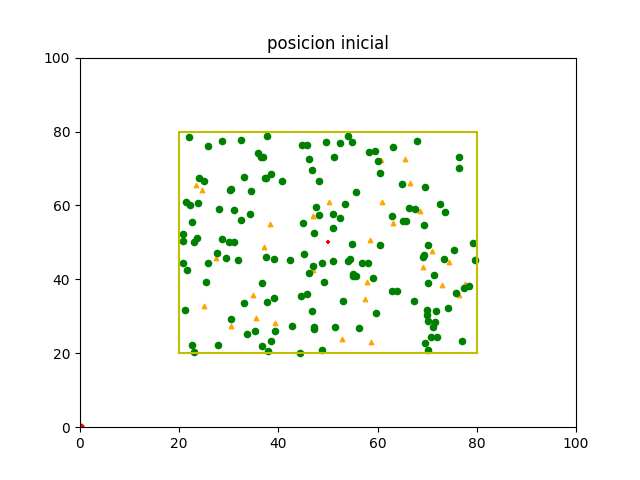
\includegraphics[width=\columnwidth]{p_inicial.png}
  \caption{Plano bidimensional de partículas de material base (puro).}
  \label{f2}
\end{figure}
\bigskip

Como siguiente propuesta para poder recaudar datos de diversos casos según los objetivos, se hace adición para generar aleaciones con partículas cerámicas, polímeros y un material conductor (plata), estas adiciones tienen fuerzas diferentes por partícula (figura \ref{f2} triángulos naranjas) que se interponen al paso de la temperatura según sus propiedades y ésta variación es la que se estudiará. Esta experimentación de las propuestas puede ser visto en el repositorio de Samaniego \cite{Edson} donde se realizaron animaciones \cite{GIPHY} para ver el movimiento de la partícula de calor a través del material.

\subsection{Experimentación}
Para la experimentación en base a las propuestas ya se tiene las aleaciones y como la temperatura penetra el material a velocidades distintas según sea el porcentaje de partículas agregadas como dopaje y la otra variante es el valor de la temperatura que en la propuesta es fijo en (45 grados). Entonces lo que se realiza después es automáticamente el cambio de temperaturas para obtener una serie de resultados en el que podamos observar para cada aleación a que temperatura se llega al punto de fusión tal como puede ser observado en la figura \ref{fig3} a) se puede ver que para el material puro a baja temperatura de setenta y cinco grados llego a su punto de fusión cero ya que es un material no dopado por otro material, pero cuando se realiza una aleación con un cerámico (material aislante) se observa que para llegar a su punto de fusión se tiene que ir aumentando mas la temperatura, le es más difícil el paso de temperatura a través de la aleación debido a sus propiedades. Mientras que para la aleación polimérica y conductora (plata) si retarda la llegada a su punto de fusión siendo este a una temperatura aproximada de ciento setenta para llegar a deformar o derretir.
\begin{figure}[H]
\centering
\begin{subfigure}[b]{1\linewidth}
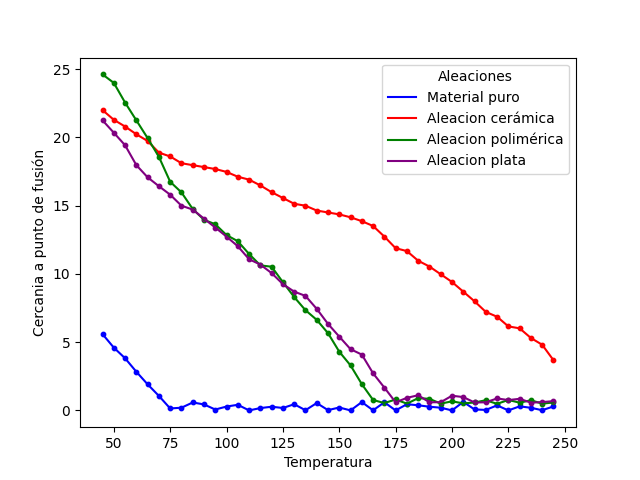
\includegraphics[width=\columnwidth]{temp_vari.png}
\caption{Gráfico de aleaciones variando temperatura con respecto al punto de fusión.}
\end{subfigure}
\begin{subfigure}[b]{1\linewidth}
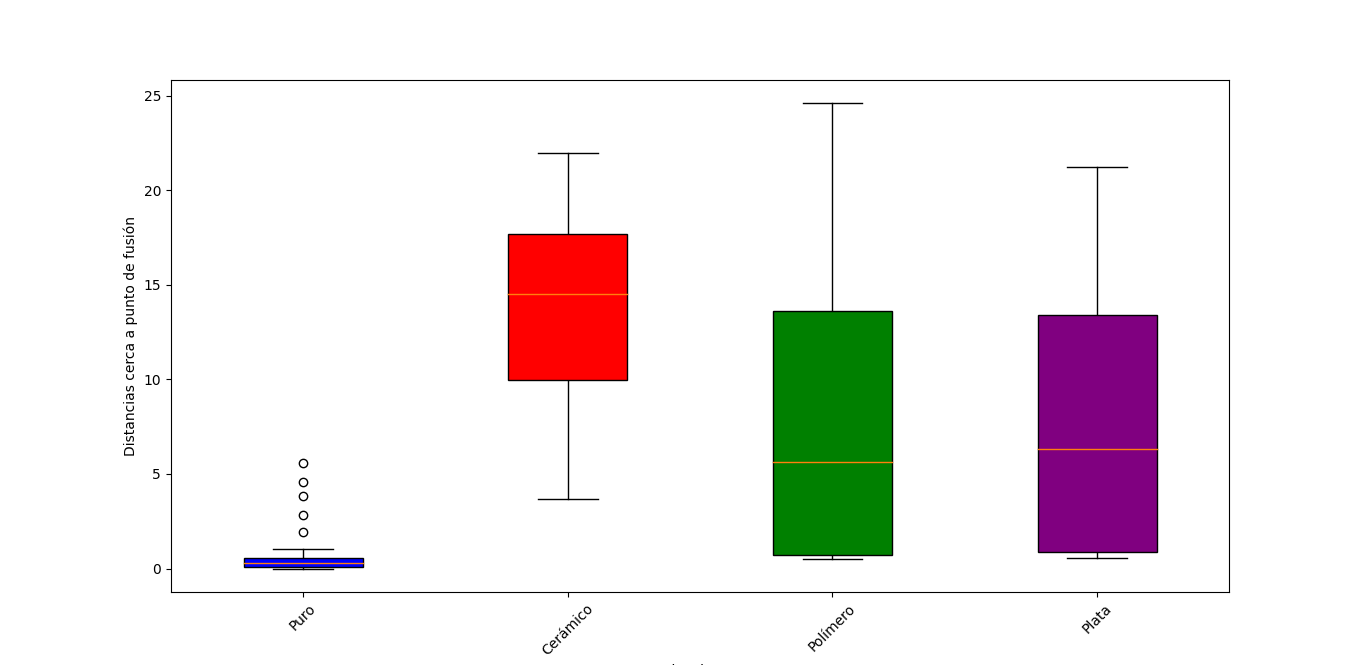
\includegraphics[width=\columnwidth]{cb_temp_vari.png}
\caption{Caja-bigote de resultados respecto a la distancia cercana al punto de fusión.}
\end{subfigure}
\caption{Gráficas de prueba realizada en diferentes aleaciones variando la temperatura.}
\label{fig3}
\end{figure}

En la figura \ref{fig3} b) puede observarse un diagrama caja-bigote que representa los resultados del punto máximo que alcanzo cada material respecto a la variación de temperatura.
Viendo este tipo de comportamiento con la temperatura ya es posible darse una idea de las propiedades que tiene cada material y en base a esto es como se desarrolla la simulación en el que ahora los parámetros a variar no son los de temperatura sino que se varía el tamaño de la masa o partícula de aleación y material puro para ver si este tiene efecto en la llegada al punto de fusión y de igual manera variar la masa de la partícula para ver el comportamiento eléctrico ya que se espera que al ser un material conductor como la plata, al tener mas tamaño de partícula de este entonces presente mayor conductividad, caso contrario con aleación cerámica que es un material aislante. 

\section{Evaluación}\label{intr}
Recordando el presente trabajo pretende examinar el comportamiento de las aleaciones cuando se varía un parámetro como lo es la masa de la partícula para ver que efecto tiene sobre cada muestra con respecto al punto de fusión del material ya que para ciertos casos se busca que un material tenga alto punto de fusión y buena conductividad (óptimo) pero todo depende la aplicación que se le de. Para la validación de la simulación los resultados pueden consultarse en el repositorio de Samaniego \cite{Edson} pero pueden ser visualizados gráficamente en la figura \ref{fig4} donde se puede observar la segunda prueba realizada que es variando la masa de la aleación dada en micrómetros teniendo un rango de partícula entre \texttt{0.05 y 0.30} convirtiéndolo obtenemos partículas de cincuenta a trescientos nanómetros. Se puede ver que la variación de tamaño de partícula hace que aumente la distancia al punto de fusión lo cual es bueno para lo que se busca analizar viendo que el material puro tiene un cambio drástico alejándolo de su punto de fusión que era cero cuando la partícula medía cincuenta nanómetros y en el material cerámico sabiendo que tiene buena conductividad térmica este se mantiene en rangos de treinta y cinco a cuarenta y cinco lo cual lo aleja más del punto de fusión,se vuelve más difícil el deformarlo debido al incremento de la partícula.
\begin{figure}[H]
\centering
\begin{subfigure}[b]{1\linewidth}
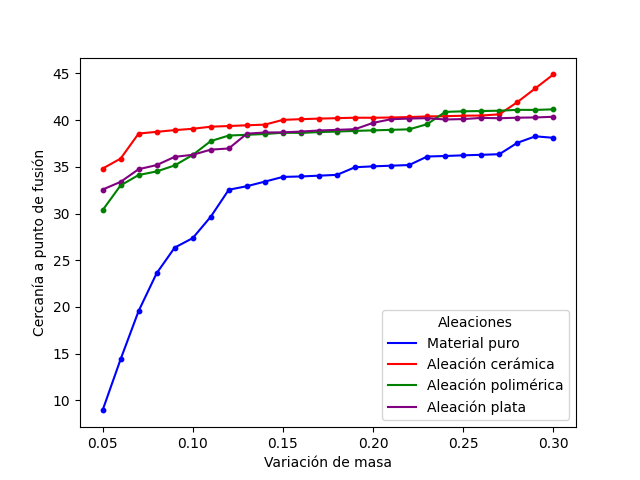
\includegraphics[width=\columnwidth]{temp_masa.png}
\caption{Gráfico de aleaciones variando masa con respecto al punto de fusión analizando conductividad térmica.}
\end{subfigure}
\begin{subfigure}[b]{1\linewidth}
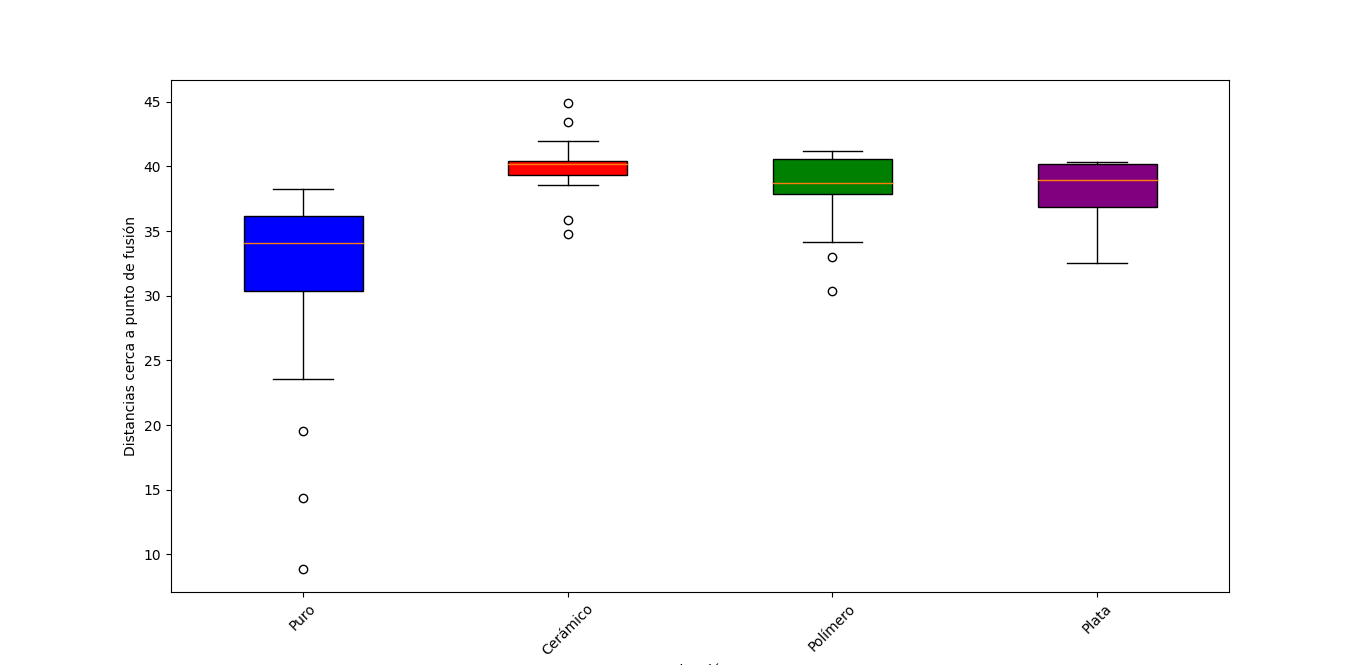
\includegraphics[width=\columnwidth]{CB_temp_masa.png}
\caption{Caja-bigote de resultados respecto a la distancia cercana al punto de fusión.}
\end{subfigure}
\caption{Análisis térmico de prueba realizada en diferentes aleaciones variando masa.}
\label{fig4}
\end{figure}

El otro objetivo es el análisis del flujo eléctrico que puede ser observado en los gráficos de la figura \ref{fig5} en el cual lo esperado es que conforme se aumenta el tamaño de la partícula de un material conductor, el flujo eléctrico se haga mayor al contrario de cuando aumentamos la partícula de cerámica  la conductividad no debe ser mayor.
Viendo el gráfico \ref{fig5} a) es posible notar que en efecto la conductividad eléctrica le favorece en mayoría a un material conductor siendo este caso ejemplo la plata la cual incremento conforme crecía la partícula.
En cuanto al material cerámico hay una variación notando un aumento pero sigue estando por debajo de un material puro y un polímero haciéndolo el de más baja conductividad (aislante). 

\begin{figure}[H]
\centering
\begin{subfigure}[b]{1\linewidth}
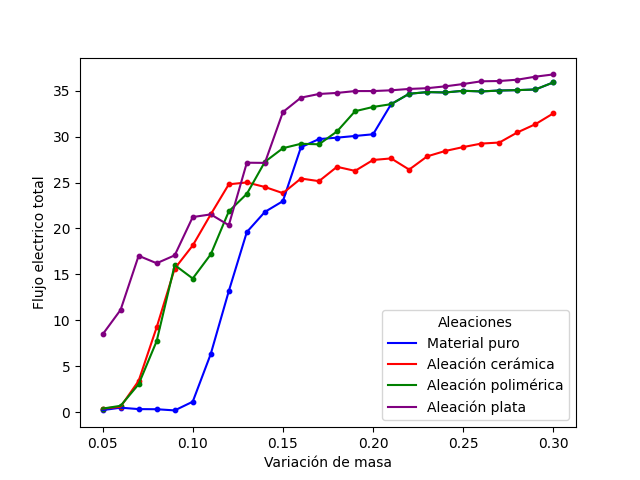
\includegraphics[width=\columnwidth]{elec_masa.png}
\caption{Gráfico de aleaciones variando masa con respecto al flujo eléctrico.}
\end{subfigure}
\begin{subfigure}[b]{1\linewidth}
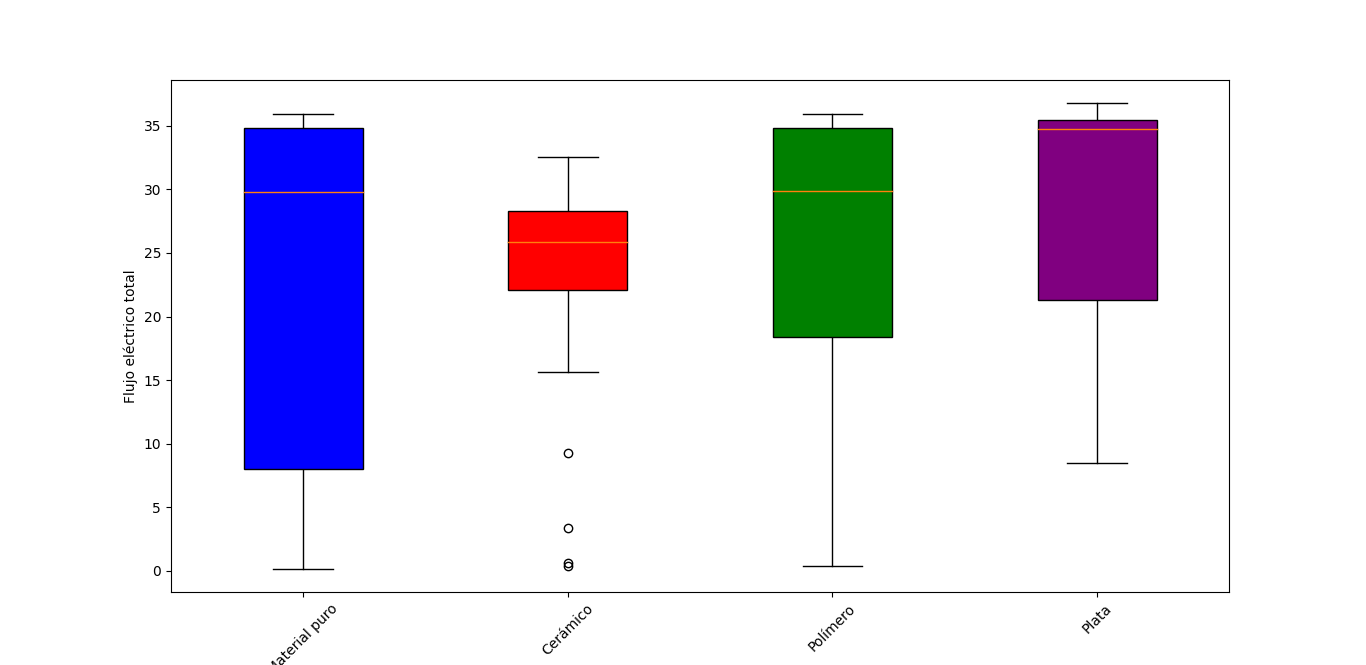
\includegraphics[width=\columnwidth]{CB_elec_masa.png}
\caption{Caja-bigote de resultados respecto a la distancia cercana al máximo flujo eléctrico.}
\end{subfigure}
\caption{Análisis eléctrico de prueba realizada en diferentes aleaciones variando masa.}
\label{fig5}
\end{figure}

La tabla \ref{tab1} engloba los resultados obtenidos en el cual es de manera sencilla identificar los valores graficados anteriormente, donde ya son distribuidos por cada aleación y tomando un valor mínimo, medio y máximo de tamaño de partícula así mismo viendo lo lejano al punto de fusión y el flujo eléctrico.

Recalcando que un valor óptimo para este caso es buscar alto punto de fusión y buena conductividad, observando que un material cerámico presenta alto punto de fusión  pero la plata presenta el mejor valor de flujo eléctrico siendo un conductor.

\begin{table}[H]
        \caption{Registro de cada aleación según su porcentaje, distancia máxima al centro(punto de fusión) y tiempo que recorrió.}
        \bigskip
        \label{tab1}
        \centering
        \begin{adjustbox}{width=\columnwidth,center}
        \begin{tabular}{|r|r|r|r|}
        \hline
         \begin{turn}{60}Aleación\end{turn}&
         \begin{turn}{60}Masa\end{turn}&
         \begin{turn}{60}Punto de fusión\end{turn}&
         \begin{turn}{60}Flujo eléctrico\end{turn} \\
        \hline
              & 0.05 &8.90&0.21   \\
        Puro  & 0.15 &33.91&22.98 \\
              & 0.30 &38.10&35.92 \\
        \hline
              & 0.05  &34.81& 0.37  \\
        Cerámico& 0.15 &40.02&23.85 \\
              & 0.30 &44.90&32.55 \\
        \hline
              & 0.05  &30.34& 0.38   \\
        Polímero& 0.15 &38.65& 28.74\\
              & 0.30 &41.16&35.92 \\
        \hline
              & 0.05 & 32.56 &8.45\\
        Plata & 0.15 &38.69& 32.68\\
              & 0.30 &40.36&36.78 \\
        \hline
        \end{tabular}
        \end{adjustbox}
    \end{table}
    
\section{Conclusiones}\label{intr}
Se conoce a ciencia cierta que un material o aleación no tienen una temperatura de fusión única, dependiendo de la concentración, cada elemento puro funde a una temperatura. Es interesante recalcar como diferentes aleaciones afectan tanto al punto de fusión de un material como su respuesta al flujo eléctrico, para análisis computacional se simuló un código que arroja respuesta gráfica de estos mismos comportamientos o fenómenos que ocurren pero a nivel nanométrico simulando la variación de masas de las partículas del material aleado. 
Obteniendo un resultado favorable al comportamiento tanto térmico como eléctrico viendo que en ambos casos el aumento de partícula favorece en relación que se aleja de su punto de fusión y aumenta el flujo eléctrico todo esto porcentualmente al tipo de aleación ya que se contiene materiales aislantes y conductores así polímeros. Denotando que el mejor material para este caso puede ser un polímero de tamaño de partícula de trescientos nanómetros el cual tiene una parte buena en conducción térmica así como buen flujo eléctrico ubicándolo gráficamente entre el cerámico y la plata.

\subsection{Trabajos futuros}
Cabe mencionar que para ésta simulación hace falta tomar en cuenta varios parámetros y propiedades del mismo material, de la misma forma incorporar valores más específicos de cada partícula de dopaje para tener mejor precisión en los resultados que requiere de una experimentación mas amplia y detallada. 

Con el desarrollo de este código como aplicación puede ser beneficioso a la hora de querer tratar un material y querer saber que características térmicas y conductivas se requieren de el para saber cuanta resistencia a la temperatura tendrá, o si es beneficioso en flujo eléctrico.

\bibliographystyle{plainnat}
\bibliography{refe}

\end{document}